\documentclass[12pt]{article}

% Packages
\usepackage[margin=1in]{geometry}
\usepackage{enumerate}
\usepackage{braket}
\usepackage{MnSymbol}
\usepackage{amsthm}
\usepackage[mathscr]{euscript}
\usepackage{graphicx}

% Definitions
\newtheorem{theorem}{Theorem}
\DeclareMathOperator*{\expected}{E}
\DeclareMathAlphabet\mathbb{U}{msb}{m}{n}

% Metadata
\title{An Introduction to Quantum Money}
\author{Niall Wingham (20228078 -- CS467)}
\date{April 13, 2013}

\begin{document}
\maketitle

\begin{abstract}
The goal of this paper is to provide an overview of the field of quantum money, from its invention to current results.  We discuss the motivation and history of quantum money, describe the terminology and techniques used to reason about quantum money, and present several proposed schemes for quantum money.  Finally, we show two promising implementations based on these schemes and investigate their security.
\end{abstract}



\section{Introduction}
The \emph{No-Cloning Theorem} states that it impossible to make perfect replicas of arbitrary quantum states.  It is a fundamental result, following from the linearity of quantum mechanics, and it highlights an important distinction: while it is easy to copy classical information, it is impossible to do so for quantum information.  This raises interesting possibilities for cryptography.  Are there tasks which are impossible using classical information, but which can be accomplished using quantum information?  One such task is to create better kinds of money.

\subsection{Motivation}
Consider the kinds of money we currently use.  Some are \emph{physical} currencies like coins and bills, or even raw commodities like gold and diamonds.  They have two disadvantages: first, they are possible to forge;\footnote{Many include security features, but at best these make them \emph{uneconomical} to forge.} and second, they are conspicuous to carry in large amounts.  Other types of currencies are \emph{digital}, like debit and credit cards, or PayPal accounts.  Because digital information can be copied freely, transactions with these currencies must be verified by some third-party authority.  This leads to two new disadvantages: first, they generally require an online connection to use; and second, they are not anonymous.

An ideal currency would combine all the benefits of these two kinds of currencies with none of the defects.  It would be unforgeable, inconspicuous, anonymous, and verifiable by anyone.  This is precisely the objective of quantum money, and current results suggest it is possible.  To be fair, we are still far from able to maintain coherent quantum states for long periods of time outside laboratory conditions, which we would need to do for real quantum money.  But that is no reason to delay development of the theory!

\subsection{Challenges}
Providing a method for anyone to verify quantum money also means providing counterfeiters a powerful tool with which to forge money.  If nothing else, a counterfeiter can run a random brute force search against a verifier, though this would succeed with exponentially small probability and is not a serious concern.  More worrying is that the counterfeiter will be able to exploit some underlying structure in the verifier to succeed in forging money in polynomial time.

A second challenge in the field of quantum money is that it is very hard to reason about security results.  The best that can be said of most current proposals is that a few people tried to break them and have not yet succeeded.  This is far from the standard we would like to hold ourselves to.

\subsection{Outline}
Our paper proceeds as follows.  In Section 2, we give a history of early work in quantum money.  In Section 3, we outline modern terminology and important theorems used to reason about quantum money.  In Section 4, we describe three frameworks for quantum money: these are abstract schemes that rely on black boxes or oracles, but which are still useful as templates.  Finally, in Section 5, we investigate the two most promising concrete implementations of quantum money.



\section{History}
The problem of quantum money was introduced by Wiesner in 1969 \cite{Wie83}.\footnote{Despite being a remarkable paper, the field of quantum information did not yet exist, and it remained unpublished for over a decade.}  He observed that if a bank prepared a piece of money as one of the states $\{\Ket{0},\Ket{1},\Ket{+},\Ket{-}\}$, it would be able to verify the state by measuring it in either the computational or Hadamard basis.  To remember which basis to use and what result it expected, the bank would keep a secret database and distribute each piece of money with a serial number $s$ linking to its record in the database.  An adversary trying to copy the money would have to guess which basis to measure it in and could only succeed with probability $3/4$: half the time they would use the correct basis and make a perfect copy, and half the time they would use the wrong basis and make a copy that would pass verification with probability $1/2$.  By using many such qubits for a single piece of money, the bank could make its money arbitrarily hard to copy.  This was the first example of a private key scheme, though it required the bank to store a database that grew linearly with the size of its money supply.

\begin{figure}[h!]
\caption{Wiesner's Quantum Money}
\Large \centering
$\Ket{\$} = \Ket{s}\Ket{\updownarrow \neswarrow \nwsearrow \leftrightarrow \leftrightarrow \nwsearrow \leftrightarrow \neswarrow \nwsearrow \nwsearrow \updownarrow \neswarrow \updownarrow \leftrightarrow \neswarrow \nwsearrow \updownarrow \leftrightarrow \updownarrow \neswarrow}$
\end{figure}

Bennett, Brassard, Breidbart, and Wiesner continued this work in \cite{BBBW83}.  For the private key scheme, they replaced the database with a secret key and pseudorandom function.  They also developed a public key scheme that was based on the difficulty of factoring large numbers (though we now know this is not hard for quantum adversaries).

It was later found (e.g. by \cite{Aar12} and \cite{Lut10}) that Wiesner and BBBW's schemes suffered from a serious flaw that allowed counterfeiters to copy money in linear time.  It uses the fact that their qubits are independent, and that successful measurements project the qubits onto a valid state.  Given a valid piece of money, a counterfeiter can swap out the first qubit with a new one in a random orientation and verify the altered bill, trying multiple times if necessary until it is accepted (it will pass with probability $1/2$).  Now he has an entirely valid bill, and a copy of the first qubit for a valid bill.  The counterfeiter proceeds in this manner along the chain of qubits until he has copied the entire piece of money.

These schemes laid an important foundation: both their construction and their flaws, though relatively simple, are illustrative of modern quantum money.  However, research in this area lay dormant for several decades.  It was not until circa 2005 that the question of quantum money was revisited, this time by researchers at MIT and the University of Waterloo.



\section{Preliminaries}
One of the first tasks for these researchers was to formalize terminology and techniques for reasoning about quantum money.  Here we introduce vocabulary that will help us describe quantum money schemes, and theorems that will help us prove results about them.  This high-level overview should also help to understand the original papers in which these schemes are presented.

\subsection{Terminology}
There is not yet consistent terminology in the literature on quantum money.  For the sake of discussing various papers together, we attempt to provide some general definitions and apply them to each one, even where it is anachronistic.  Most come from Aaronson, who formalized them in \cite{Aar09} and \cite{Aar13}, but we take e.g. collision-freedom from Lutomirski et al. in \cite{Lut09} and anonymity from Mosca and Stebila in \cite{Mos10}.

\begin{description}
\item[Quantum Money] A piece of quantum money $\Ket{\$} = \Ket{s}\Ket{\$_s}$ consists of a serial number $\Ket{s}$ and a corresponding quantum state $\Ket{\$_s}$.
\item[Schemes] A quantum money scheme $\mathscr{S}$ consists of two polynomial-time algorithms: a producer $P$ and a verifier $V$.  $P\Ket{0} = \Ket{\$}$ creates new pieces of money, and $V\Ket{s}\Ket{\psi} = Accept$ or $Reject$ validates alleged pieces of money.  An issuing bank may also digitally sign its money to distinguish it from other banks or counterfeiters who implement the same scheme.
\item[Private Key] In a private key scheme, some secret is needed in order to run $V$.  Typically, this secret is known only by the issuing bank.  We are less interested in private key schemes because offline verifiability is an important goal of quantum money.
\item[Public Key] In a public key scheme, anyone can run $V$.  Public key schemes may be computationally secure, but they cannot be information-theoretically secure.  With access to $V$, a counterfeiter can always run a brute force search for valid pieces of money.
\item[Completeness] For all valid pieces of money $\Ket{\$}$, we say a scheme has \emph{completeness error} $\varepsilon$ if $V\Ket{\$}=Reject$ with probability $\varepsilon$.  If $\varepsilon=0$, we say the scheme is \emph{complete}.
\item[Soundness] For any counterfeiting algorithm $C$, which is allowed as input several valid pieces of money $\{\Ket{\$_0},...,\Ket{\$_k}\}$, we say a scheme has \emph{soundness error} $\delta$ if $C$ can produce a new state $\Ket{\$_{k+1}}$ such that  $V\Ket{\$_{k+1}}=Accept$ with probability $\delta$.  If $\delta=0$, we say the scheme is \emph{sound}.\footnote{A counterfeiter can be allowed at most polynomially many pieces of money, or else an attack using quantum state tomography is possible.}
\item[Collision-Freedom] A scheme is \emph{collision-free} if $P$ cannot produce two identical pieces of money.  In such a scheme, rather than digitally signing its money, an issuing bank could simply publish a list of the serial numbers for the money it has produced.\footnote{Using this kind of verification also has the side effect, pointed out in \cite{Lut09}, of making it impossible for an issuing bank to secretly inflate the money supply by creating two pieces of money with the same serial number.  Of course, a bank could still secretly deflate the money supply by publishing more serial numbers than it had actually produced.}
\item[Anonymity] A scheme is \emph{anonymous} if every piece of money produced by $P$ is identical.  In this type of scheme, no piece of money can be tracked.  This is the opposite of a collision-free scheme.
\end{description}

\subsection{Techniques}
Aaronson has also made significant contributions to formalizing the security of quantum money schemes.  Indeed, most other published schemes rely on his techniques to prove their security.  Here we present four of his important results as theorems and describe their meaning and application to quantum money.

\begin{theorem}[Almost As Good As New]
Suppose a measurement on a mixed state $\rho$ yields a particular outcome with probability $1 - \varepsilon$.  Then after the measurement, one can recover a state $\tilde{\rho}$ such that $\|\tilde{\rho} - \rho\|_\mathrm{tr} \leq \sqrt{\varepsilon}$.
\end{theorem}

This result, given as a lemma in \cite{Aar05}, says that if we know enough about a quantum state to predict its measurement with high confidence, then measuring it will damage it only slightly.  It is used to prove that valid pieces of quantum money can be verified and re-used many times provided the scheme has negligible completeness error.

\begin{theorem}[Quantum-Secure Signature Schemes]
If there exists a (classical) one-way function f secure against quantum attack, then there also exists a digital signature scheme secure against quantum chosen-message attacks.
\end{theorem}

This theorem is given in \cite{Aar13}.  It suggests that although many current digital signatures (e.g. those based on RSA) are not secure against quantum adversaries, it is possible to construct new signatures which are.  It allows us to talk about digital signatures in general with some degree confidence, for example, when we said in Section 3.1 that an issuing bank should sign the money it produces.

\begin{theorem}[Complexity-Theoretic No-Cloning]
Let $\Ket{\psi}$ be an $n$-qubit pure state.  Suppose we are given the state $\Ket{\psi}^{\otimes k}$ for some $k \geq 1$, as well as an oracle $U_\psi$ such that $U_\psi\Ket{\psi} = -\Ket{\psi}$ and $U_\psi\Ket{\phi} = \Ket{\phi}$ for all $\Ket{\phi}$ orthogonal to $\Ket{\psi}$.  Then for all $\ell > k$, to prepare $\ell$ registers $\rho_1,...,\rho_\ell$ such that $$\sum_{i=1}^\ell\Bra{\psi}\rho_i\Ket{\psi} \geq k + \delta,$$ we need $$\Omega\left(\frac{\delta^2\sqrt{2^n}}{\ell^2k\log{k}} - \ell\right)$$ queries to $U_\psi$.
\end{theorem}

This theorem is claimed in \cite{Aar09} though only a sketch of its proof was offered until \cite{Aar13}.  If a counterfeiter attempts to copy one or more pieces of money without using the scheme's verifier, then the no-cloning theorem applies.  Alternately, if a counterfeiter attempts to find a valid piece of money by consulting the scheme's verifier, but without using any existing pieces of money, then the lower bound for quantum search applies.  However, a real counterfeiter will take advantage of both.  This theorem shows he still cannot do much better than guessing, as long as there is no underlying structure in the verification algorithm that he can exploit.  It is used to prove that oracle-based quantum money schemes have negligible soundness error.

\begin{theorem}[Inner-Product Adversary Method]
For some quantum algorithm $Q$ and classical oracle $U$, let $\Ket{\Psi^U_t}$ be $Q$'s state after $t$ queries to the oracle.  Given:

\begin{enumerate}[(i)]
\item A set of quantum oracles $\mathscr{O}$ with every $U \in \mathscr{O}$ having a subspace $S_U \leq \mathscr{H}^{2^n}$ such that $U\Ket{\psi} = -\Ket{\psi}$ for all $\Ket{\psi} \in S_U$, and $U\Ket{\phi} = \Ket{\phi}$ for all $\Ket{\phi} \in S_U^\perp$
\item A symmetric irreflexive binary relation $\mathscr{R}$ with every $U \in \mathscr{O}$ having at least one $V \in \mathscr{O}$ such that $(U,V) \in \mathscr{R}$
\end{enumerate}

\noindent Suppose that for every $U \in \mathscr{O}$ and all $\Ket{\phi} \in S_U^\perp$, we can show:\footnote{Where $\expected $ is the expected value and $F$ is fidelity.  Fidelity is a measure of the closeness of a mixed state to another mixed state or a subspace, but it is beyond the scope of this paper to formally introduce it; for more details see \cite{Aar13}, \S~2.2.}

$$\expected_{V : (U,V) \in \mathscr{R}} \left[F\left(\Ket{\phi},S_V\right)^2\right] \leq \varepsilon$$

\noindent Furthermore, suppose that for all $(U,V) \in \mathscr{R}$, when $Q$ starts we have $\left[\Braket{\Psi^U_0 | \Psi^V_0}\right] \geq c$, and when $Q$ finishes we have $\left[\Braket{\Psi^U_0 | \Psi^V_0}\right] \leq d$.  Then $Q$ must make at least $\Omega\left((c - d) / \varepsilon\right)$ oracle queries.
\end{theorem}

This theorem is given in \cite{Aar13} and is used to prove the security of Aaronson's oracle-based quantum money scheme as well as the Complexity-Theoretic No-Cloning Theorem.  The idea behind it is to give an upper-bound for how well a quantum algorithm can distinguish pairs of oracles as the result of a single query.

Ideally, we would be able to show that the inner product $\left[\Braket{\Psi^U_0 | \Psi^V_0}\right]$ decreases by at most $\varepsilon$ with each query, in which case it easily follows that we need to make $\Omega((c-d)/\varepsilon)$ queries to reduce the inner product from $c$ to $d$.  However, it is not generally possible to show this for quantum money schemes since $Q$ also has information beyond the oracles, in the form of valid pieces of money.  Instead, we have to examine how much the inner product is \emph{expected} to decrease with each query, for some carefully designed distribution of oracle pairs $(U,V)$.



\section{Frameworks}
We are now ready to examine three framework schemes for public key quantum money.  We call them frameworks because each scheme is dependent on one or more black box oracles that recognize special states by flipping their phase (that is, the recognized state is a $-1$ eigenstate of the oracle).

Recall that in Section 3.1, we saw that some scheme properties conflict with each other.  In particular, a scheme cannot be both \emph{anonymous} and \emph{collision-free}.  In physical currencies, coins are indistinguishable from each other while bills are printed with serial numbers.   Therefore, we say anonymous schemes make \emph{quantum coins} while non-anonymous schemes make \emph{quantum bills}.

It is beyond the scope of this paper to prove it, but all of the following schemes are complete and with negligible soundness error.  The proof for each scheme can be found in the paper in which the scheme was introduced, and should be somewhat familiar based on the techniques introduced in Section 3.2.

\subsection{Quantum Coins}
The only published framework for public key quantum coins comes from Chapter 8 of Stebila's thesis \cite{Ste09}, also presented in \cite{Mos06} and \cite{Mos10}.  To create coins of some denomination $d$, the issuing bank randomly selects a secret pure state $\Ket{\psi_d} \in \mathscr{H}^{2^n}$ and uses an oracle $U_{\psi_d} = I - 2\Ket{\psi_d}\Bra{\psi_d}$.  Note that this oracle recognizes exactly $\Ket{\psi_d}$ by flipping its phase, similar to an oracle for amplitude amplification.  The quantum coin scheme $\mathscr{S}_d = (P,V)$ is then formally defined by:

\begin{align*}
P\Ket{0} & = \Ket{d}\Ket{\psi_d} = \Ket{\$_d}\\
V\Ket{\$_d} & = \left\{
	\begin{array}{l l}
	Accept & \text{if $U_{\psi_d}\Ket{\$_d} = -1$}\\
	Reject & \text{otherwise}
	\end{array}
\right.
\end{align*}

Note that the ``serial number'' slot of the money is effectively ignored; we include it for the sake of having a consistent definition of quantum money.

\subsection{Quantum Bills}
There are two recent frameworks of interest for public key quantum bills, one proposed by Lutomirski et al. in \cite{Lut09}, and the other by Aaronson and Christiano in \cite{Aar13}.  The former scheme is collision-free but requires an oracle which seems more difficult to implement.  Both of these schemes involve states that are uniform superpositions over sets.  For notational simplicity, we define $$\Ket{S} := \frac{1}{\sqrt{|S|}} \sum_{s \in S} \Ket{s}$$

\subsubsection{Quantum Money by Postselection}
The idea behind the first scheme is to create a uniform superposition over a large, randomly selected set, with a serial number identifying which set was chosen.  To verify a piece of alleged money, an oracle checks that the state is a uniform superposition over the correct set.

Let $S$ be the set of $n$-bit strings, and let $L$ be a ``labelling function" which assigns a label $\ell$ to each $s \in S$.  Finally, let ${S_\ell} = \{s : L(s) = \ell\}$ be the set of elements for a given label.  $L$ should be constructed so that there are exponentially many different labels, and so each $S_\ell$ has exponentially many elements; it should also have as little structure as possible.  Finally, we require oracles $U_\ell$ which recognize states in a uniform superposition over $S_\ell$.

The production algorithm $P$ is defined by the following three steps.  First, it generates a uniform superposition over $S$.  Then, it applies the labelling function to the superposition to obtain an augmented superposition.  Finally, it measures the value of $L$ to collapse the state to a superposition over a particular $S_\ell$.  A piece of money $\Ket{\$_\ell}$ looks like $\Ket{\ell}\Ket{S_\ell}$.

\begin{figure}[h!]
\caption{Production by Postselection}
\centering
$\displaystyle
\frac{1}{\sqrt{|S|}} \sum_{s \in S} \Ket{0}\Ket{s} \quad
\Rightarrow \quad
\frac{1}{\sqrt{|S|}} \sum_{s \in S} \Ket{L(s)}\Ket{s} \quad
\Rightarrow \quad
\frac{1}{\sqrt{|S_\ell|}} \sum_{s \in S_\ell} \Ket{\ell}\Ket{s}
$
\end{figure}

Given an alleged piece of money $\Ket{\$} = \Ket{\ell}\Ket{\psi}$, the verification algorithm $V$ is defined by the following two steps.  First, it checks that $L\Ket{\psi} = \ell$.  Second, it checks that $U_\ell\Ket{\psi} = -\Ket{\psi}$.  If both of tests pass, $P\Ket{\$} = Accept$; otherwise $P\Ket{\$} = Reject$.

Lutomirski et al. propose that the oracles $U_\ell$ could be implemented using a special Markov matrix which rapidly mixes any distribution of strings $S_\ell$ to the uniform distribution $\Ket{S_\ell}$, but does not mix between strings with different labels.  Each update in the Markov chain would consist of a random choice between $N$ unitary update rules.  Then, any valid $\Ket{\psi_\ell}$ is a $+1$ eigenstate of $M$, and $M^r$ approximates a projection onto $\Ket{S_\ell}$.

\subsubsection{Quantum Money from Hidden Subspaces}
The idea behind the second scheme is to create superpositions over subspaces $A \leq \mathbb{F}_2^n$, with a serial number identifying the subspace for each bill.  To verify a piece of alleged money, an oracle checks that a state is a uniform distribution over the correct subspace.

Let the generator $G$ be a function which takes a random seed $r$ and outputs a list of linearly independent generators $\Braket{A_r} = \{x_1,...,x_{n/2}\}$ for $\Ket{A_r}$, and an identifying serial number $s_r$.  We also require oracles $U_A$ and $U_{A^\perp}$ which recognize elements of their respective subspaces (i.e. $U_A\Ket{x} = -\Ket{x}$  if $\Ket{x} \in A$ and $\Ket{x}$ otherwise).  Note that we can transform $\Ket{A}$ to $\Ket{A^\perp}$ and back again by applying a Hadamard gate to each qubit.  Also note that we can construct a projector $P_A$ onto the set of basis states in $\Ket{A}$ by initializing a control bit $\Ket{c} = \Ket{+}$, applying a controlled-$U_A$, measuring $\Ket{c}$ in the Hadamard basis, and postselecting on the outcome $\Ket{-}$.

Now we can formally define the scheme.  The production algorithm takes the following three steps.  First, it chooses a random seed $r$.  Second, it generates $G(r) = \left(s_r,\Braket{A_r}\right)$.  Finally, it outputs the money state $\Ket{\$_r} = \Ket{s_r}\Ket{A_r}$.

Given an alleged piece of money $\Ket{\$} = \Ket{s_r}\Ket{\psi}$, the verification algorithm is defined by $V_r\Ket{\psi} = H^{\otimes n} P_{A_r^\perp} H^{\otimes n} P_{A_r} \Ket{\psi}$.  It projects $\Ket{\psi}$ onto $\Ket{A}$, transforms it to the Hadamard basis and projects it onto $\Ket{A^\perp}$, and finally returns it to the standard basis.  The verifier only needs to perform two tests: this is an elegant parallel to Wiesner's original idea of quantum money based on complementary observables.

\section{Implementations}
Of course, the real challenge is to implement ones of these scheme without using an oracle.  The issuing bank must be able to distribute some obfuscated program $P$ that can take the place of its framework's oracle without revealing any kind of structure that allows counterfeiters to treat it as more than a black box.  Some previously proposed implementations, e.g. \cite{Aar09} have been shown to be insecure.  Here we examine two implementations for public key quantum bills that have not yet been broken.  The first implements the postselection scheme, and the second implements the hidden subspaces scheme.

There has not yet been a proposed implementation for quantum coins.  It seems that it is even harder to obfuscate $P$ in this case because the pieces of money it is operating on are all identical.  This gives an even larger advantage to the counterfeiter.

\subsection{Equivalent Knots}
Recall from section 4.2.1 that to implement the postselection scheme, we need to define a set $S$,  labelling function $L$, and a carefully designed Markov matrix $M$ that mixes quickly between elements sharing a label but not between others.  In \cite{Far12}, Farhi et al. build on their work in \cite{Lut09} to implement such a scheme based on the difficulty of determining if two arbitrary knot diagrams are equivalent.

We will briefly introduce some knot theory.  A \emph{knot} can be thought of as a loop of string in three dimensional space, though we usually draw knot diagrams in two dimensions.  A \emph{link} is a collection of knots, which may be tangled together.  If each knot in the link has a direction, it called an \emph{ordered link}.  Two links are equivalent if one can be ``rearranged" to be the same as the other without cutting any of the knots.  A sequence of \emph{Reidemeister moves} is sufficient to describe any valid rearrangement.  These moves are: twisting or untwisting a string; moving one string over another; and moving a string completely over or under a crossing.  Finally, the \emph{Alexander polynomial} is a polynomial which can be computed in polynomial time from an arbitrary oriented link diagram.  Equivalent knots have the same Alexander polynomial, so it is invariant under the Reidemeister moves.  (However, two knots with the same Alexander polynomial are not necessarily equivalent.)

\begin{figure}
\caption{A Knot Diagram}
\centering

\includegraphics[height=0.15\textwidth,natwidth=200,natheight=200]{trefoil_knot.png}
\end{figure}

\begin{figure}
\caption{The Reidemeister Moves}
\centering
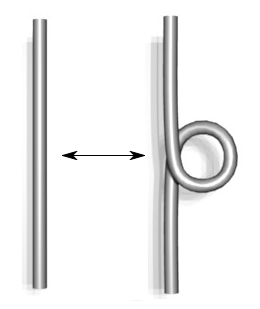
\includegraphics[height=0.15\textwidth,natwidth=260,natheight=309]{rmove1.png}
\qquad
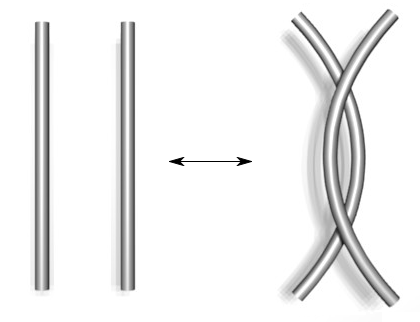
\includegraphics[height=0.15\textwidth,natwidth=420,natheight=322]{rmove2.png}
\qquad
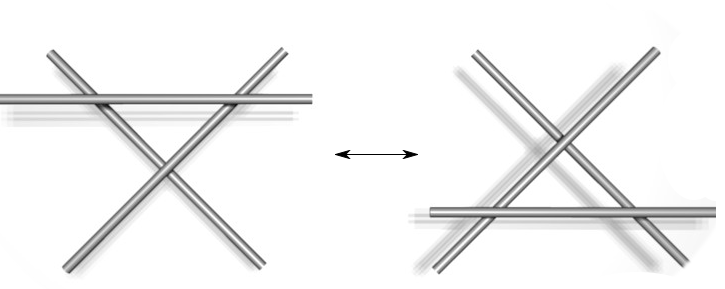
\includegraphics[height=0.15\textwidth,natwidth=725,natheight=289]{rmove3.png}
\end{figure}

Now we can describe their construction of a postselection scheme.  Let the starting set $S$ be the set of oriented links of a certain size encoded as strings in $\mathbb{F}_2^n$.  Let the labelling function $L$ be the Alexander polynomial, which divides $S$ into exponentially many groups $S_\ell$, themselves having exponentially many elements, as required.  Finally, let the Markov chain $M$ be one which at each step selects a random part of the link and applies a random Reidemeister move to it.\footnote{There are other technical details, e.g. to make sure the initial encodings are valid and that a link diagram doesn't grow too large during a Reidemeister move, but this captures the spirit of the implementation.}

If a counterfeiter were to fully measure a piece of money $\Ket{\$} = \Ket{\ell}\Ket{S_\ell}$, they would get a single link diagram $d \in S_\ell$ having Alexander polynomial $\ell$.  From there they could reconstruct a superposition of all link diagrams equivalent to $d$, which, though not equal to $\Ket{S_\ell}$, would still be a $+1$ eigenstate of $M^r$ and so would pass the verification method.  However, this would amount to solving the knot equivalence problem, which is currently thought to be hard even for quantum computers.  Farhi et al. also discuss other possible lines of attack and conclude that their scheme is probably secure, issuing the challenge, ``Forge it if you can!"

In \cite{Aar13}, Aaronson and Christiano point out some limitations of this implementation.  As shown above, states other than the ones produced by the issuing bank can pass the scheme's verification test, and simply finding out exactly which states it will accept remains an open problem that may require advances in knot theory to solve.  The implementation hasn't been broken yet, but at the same time, it is hard to say much about whether it will remain unbroken in the future.

\subsection{Multivariate Polynomials}
Recall from Section 4.2.2 that to implement the hidden subspaces scheme, we need a program $P$ that can recognize membership in $A$ and $A^\perp \leq \mathbb{F}_2^n$.  In \cite{Aar13}, Aaronson and Christiano suggest a strategy based on multivariate polynomial cryptography.

Given a set $P = \{p_1,...,p_m\}$ of multivariate polynomials from $\mathbb{F}_2^n$ to $\mathbb{F}_2$, it is hard to find a point $v \in \mathbb{F}_2$ at which $P$ vanishes; that is, at which $p(v) = 0$ for all $p \in P$.  However, given a candidate $v$, it is easy to verify that a collection of polynomials does vanish at $v$.  Therefore, for each piece of money $\Ket{\$}$ the issuing bank can provide two sets $P_A$ and $P_{A^\perp}$ of polynomials which vanish on each point of $A$ and $A^\perp$, respectively.  These sets will play the part of the oracles.

Let's see how to construct such a $P_A$.  First, note that we are evaluating a polynomial $p(x_1, ..., x_n)$ on a point $v \in \mathbb{F}_n$ by viewing $v$ as an $n$-tuple $(v_1, ..., v_n)$.  We can also restrict ourselves to \emph{multilinear} polynomials since $x^2 = x$ in $\mathbb{F}_2$.  Now consider the set $\mathscr{J}_{d,A}$ of multilinear polynomials having degree $d$ which vanish on $A$.  If the basis for $A$ is $X_A = \{x_1, ..., x_{n/2}\}$ then, every monomial of $p \in \mathscr{J}_{d,A}$ must intersect $X_{A^\perp} = \{x_{n/2 + 1}, ..., x_n\}$.  Importantly, this means we don't need to go through the expensive process of enumerating the entire set $\mathscr{J}_{d,A}$.  If all we want is to choose a random element $p \in \mathscr{J}_{d,A}$, we can simply iterate over the $O(n^d)$ possible monomials and include ones that intersect $X_{A^\perp}$ with probability 1/2.  Selecting some number $\beta$ of polynomials in this manner will give us our set $P_A$ in $O(\beta n^d)$ time.

Aaronson and Christiano also provide a method to further disguise the polynomials, by adding random noise, so only a fraction of the polynomials in $P_A$ vanish for a given point $v \in A$.  They show that the implementation remains complete even with noise added.  This gives a potential ``second chance" if the noiseless version is shown to be insecure.  Finally, they compare their hardness assumptions to well-studied and similar assumptions in multivariate polynomial cryptography, and conclude that the implementation is very likely secure when $d \geq 3$.

Other researchers have yet to critique this implementation; \cite{Aar13} is a very recent article, and no subsequent work in quantum money has yet been published.

\section{Conclusion}
We have shown two promising implementations of quantum money based on two different frameworks.  It is important to understand that even if an implementation is shown to be insecure, its underlying framework continues to be valuable.  For example, any method for distinguishing between states in a subspace $A$ and its complement $A^\perp$ would be sufficient to make money based on hidden subspaces, regardless of the security of multivariate polynomials.  This is encouraging.

Some of the open problems shift weight onto classical mathematics: we probably need to understand more about knots to prove stronger results about Farhi et al.'s proposal.  But there is also plenty of work to be done in the space of quantum information.  We expect that new frameworks and implementations based on different assumptions will continue to be created, widening the range of possibilities for a formal security result.

Then all that's left is to figure out how to actually build the darn things!


\newpage
\bibliographystyle{plain}
\bibliography{sources}

\end{document}
